\subsection*{Eskymáci} % (fold)
\label{sub:eskymáci}

\begin{multicols}{2}
	

STRAŠIDELNÁ HLÍDKA

Když jsem měla hlídku tak se ozvalo VÁŽENÍ CESTUJÍCÍ VLAK PŘIJEDE NA DRUHOU KOLEJ.

\podpis{Zub}


NA TÁBOŘE!

Jednoho dne když Kujonka a Karkulka plnili úkoli a Kujonka mlčela a karKůlka bila slepá tak si pomáhali no chápete? tak jsem jim musela pomoct já Undži
Na táboře jednoho večera sem vodešla za Kujonkou z baru ven do polotmi, Kujonka tam dělala náramky potom jsme si povídali a povídali, až najednou zničeho nic spadl obří těžký strom! Kujonka vám to může potvrdit podpisem: Kujónka

\podpis{Undži}


Nejstrašidelnější a zároveň i nejvtipnější když jsem byla na hlídce a měla jsem přepad KDE mě svalili na zem a zacpali mi pusu (dva) pak když vylezla Debat bez ponožek tak na ní šel jeden a ostatní pohazovali věci jako zprej na latry, vložky, mouku a ostatní dohromady jich bylo asi osum.

\podpis{GRIZZLY}


Na pokladovce když ještě byli všechny skupinky spolu sme se honili a kujónce se namočil šátek do marmelády. kujónka  byla nešťastná a to hodně moc a moc. všichni jsme se snažili aby nebyla smutná ale najednou se jumbo podívala na ten šátek a řekla: “kujonko, vždyť to je undžin šátek.” Všichni jsme se smáli a pak se zjistilo že kujončin šátek mám já a že ten můj leží v táboře na undží posteli takže nakonec měla špinaví šátek undži a já ho na pokladovce neměla.:)

\podpis{KARKULKA}


Na táboře byl můj nejlepší zážitek, když jsem slibovala. Můj druhý nejlepší zážitek, byly to přípravy na slib po lese byli rozmístěny svíčky s otázkami když jsem je všechny vyplnila tak jsem šla za Pískletem s otom popvídat

\podpis{Čudlík}


NEJFTIPNĚJŠÍ: KDYŽ JSEM NAPODOBOVALA SLEPICI a PÍSKLE NEČEKANĚ DALA PODEMNĚ VAJÍČKO KDYŽ JSEM UKAZOVALA JAK biSEM VISEDÁVALA VEJCE 


\podpis{KUJÓNKA}


Na pětidence jsme se večer plížili za drakem protože jsme ho chtěli zapíchnout a drak říkal: já mám hlad druhá hlavo já mám taky hlad první hlavo to bude asi tím, že máme stejný žaludek.


\podpis{gingo}

\end{multicols}

\begin{center}
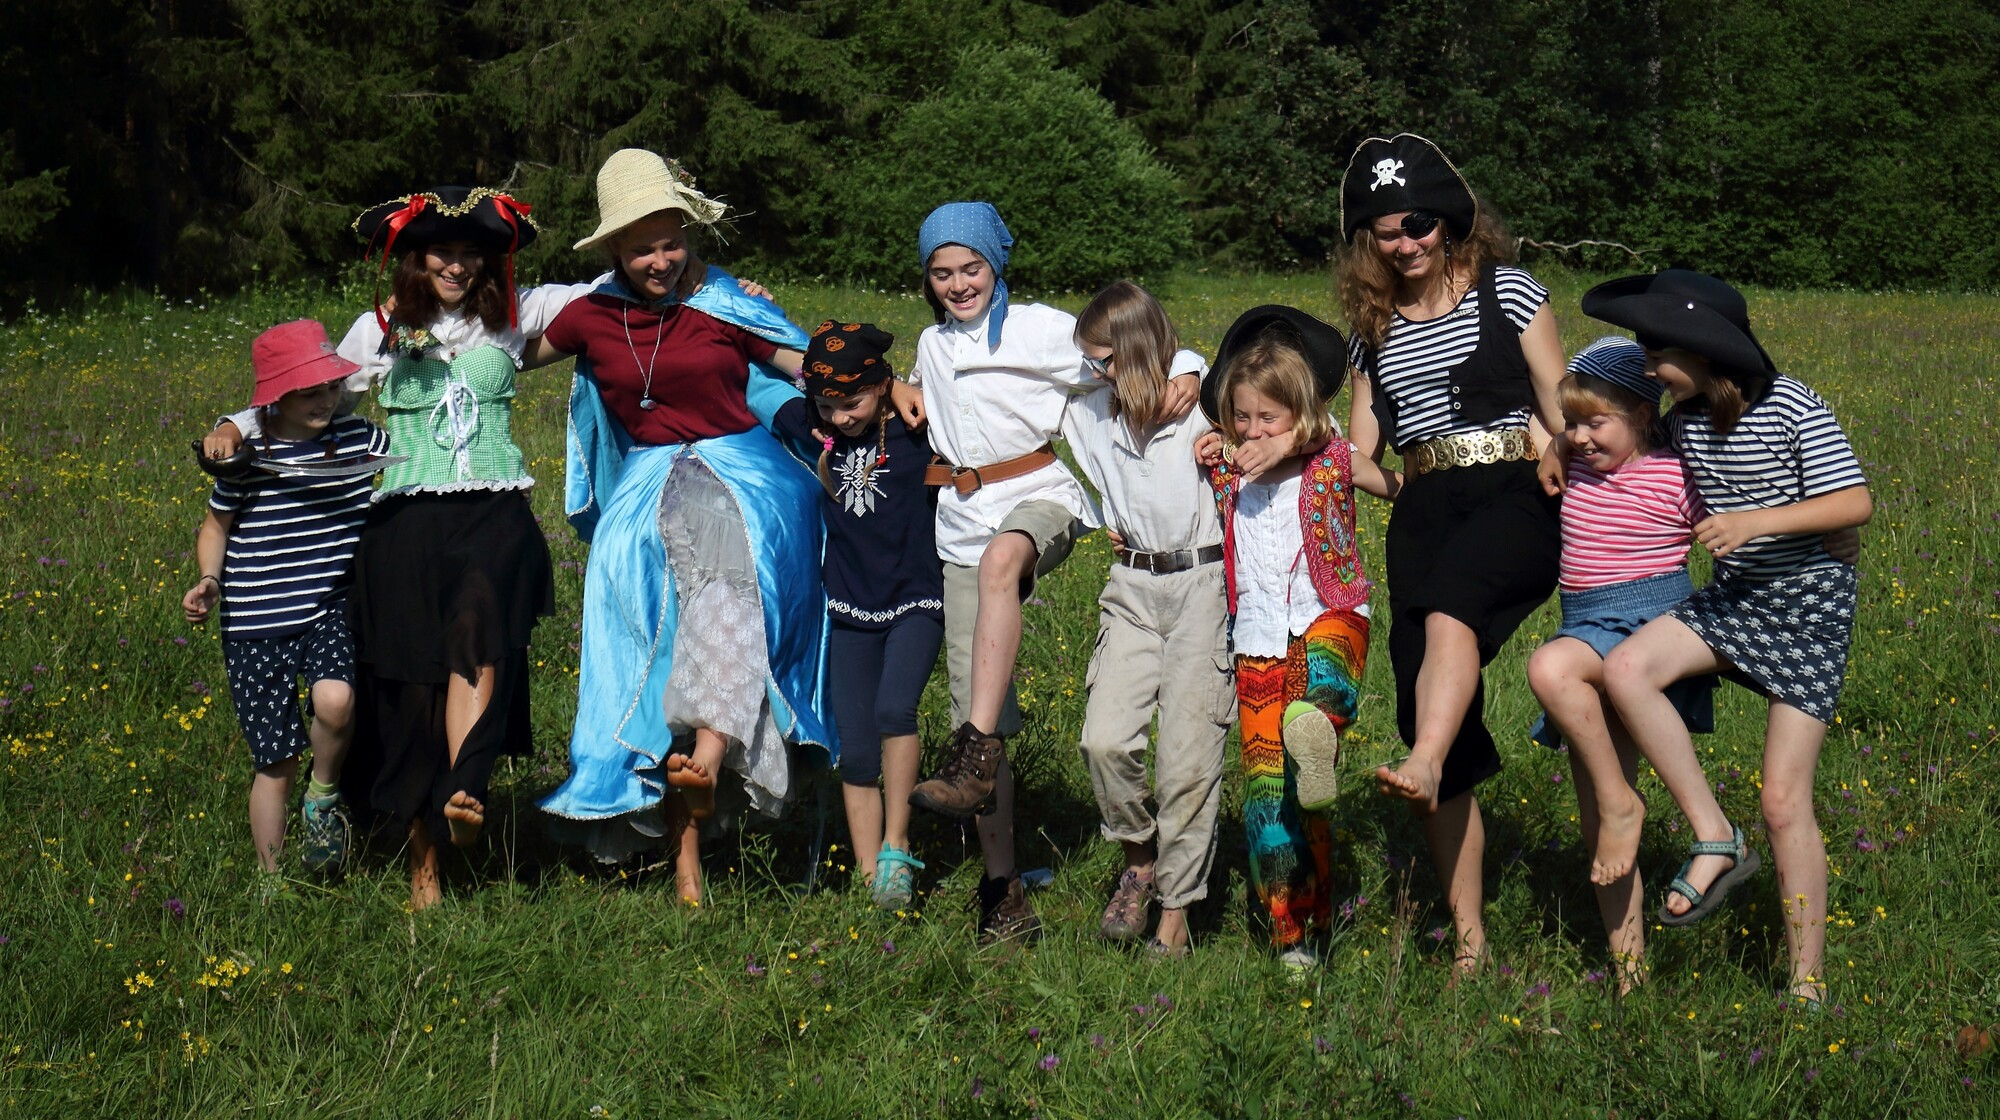
\includegraphics[width=11cm]{img/druziny/eskymaci.JPG}
\end{center}

% subsection eskymáci (end)
